% python classes slides - introduction
% (c) 2012 Kostiantyn Danylov aka koder 
% koder.mail@gmail.com
% distributed under CC-BY licence
% http://creativecommons.org/licenses/by/3.0/deed.en

\documentclass{article}
% XeLaTeX
\usepackage{xltxtra}
\usepackage{xunicode}
\usepackage{listings}
\usepackage[landscape]{geometry}

% Fonts
\setmainfont{DejaVu Sans} %{Arial}
\newfontfamily\cyrillicfont{Nimbus Roman No9 L} %{Arial}
\setmonofont{Courier New}
%\setmonofont{Ubuntu Mono}

%\setmonofont{DejaVu Sans Mono}

% Lang
\usepackage{polyglossia}
\setmainlanguage{russian}
\setotherlanguage{english}
\usepackage[dvipsnames,table]{xcolor}


\ifx\pdfoutput\undefined
\usepackage{graphicx}
\else
\usepackage[pdftex]{graphicx}
\fi

\lstset{
	language=python,
	keywordstyle=\color{Emerald},%\texttt, 
	commentstyle=\color{OliveGreen},%\texttt,
	stringstyle=\color{Bittersweet},%\texttt,
	tabsize=4,
	numbers=left,
	xleftmargin=10pt,
	morekeywords={with,as},	
	numberstyle=\large,
	%identifierstyle=\texttt,
	%basicstyle=\texttt,
}

\usepackage{hyperref}

\hypersetup{
	colorlinks=true,
	urlcolor=blue
}

\usepackage{float}
%\floatstyle{boxed} 
%\restylefloat{figure}
\usepackage[normalem]{ulem}


\makeatletter
\def\PY@reset{\let\PY@it=\relax \let\PY@bf=\relax%
    \let\PY@ul=\relax \let\PY@tc=\relax%
    \let\PY@bc=\relax \let\PY@ff=\relax}
\def\PY@tok#1{\csname PY@tok@#1\endcsname}
\def\PY@toks#1+{\ifx\relax#1\empty\else%
    \PY@tok{#1}\expandafter\PY@toks\fi}
\def\PY@do#1{\PY@bc{\PY@tc{\PY@ul{%
    \PY@it{\PY@bf{\PY@ff{#1}}}}}}}
\def\PY#1#2{\PY@reset\PY@toks#1+\relax+\PY@do{#2}}

\expandafter\def\csname PY@tok@gd\endcsname{\def\PY@tc##1{\textcolor[rgb]{0.63,0.00,0.00}{##1}}}
\expandafter\def\csname PY@tok@gu\endcsname{\let\PY@bf=\textbf\def\PY@tc##1{\textcolor[rgb]{0.50,0.00,0.50}{##1}}}
\expandafter\def\csname PY@tok@gt\endcsname{\def\PY@tc##1{\textcolor[rgb]{0.00,0.25,0.82}{##1}}}
\expandafter\def\csname PY@tok@gs\endcsname{\let\PY@bf=\textbf}
\expandafter\def\csname PY@tok@gr\endcsname{\def\PY@tc##1{\textcolor[rgb]{1.00,0.00,0.00}{##1}}}
\expandafter\def\csname PY@tok@cm\endcsname{\let\PY@it=\textit\def\PY@tc##1{\textcolor[rgb]{0.25,0.50,0.50}{##1}}}
\expandafter\def\csname PY@tok@vg\endcsname{\def\PY@tc##1{\textcolor[rgb]{0.10,0.09,0.49}{##1}}}
\expandafter\def\csname PY@tok@m\endcsname{\def\PY@tc##1{\textcolor[rgb]{0.40,0.40,0.40}{##1}}}
\expandafter\def\csname PY@tok@mh\endcsname{\def\PY@tc##1{\textcolor[rgb]{0.40,0.40,0.40}{##1}}}
\expandafter\def\csname PY@tok@go\endcsname{\def\PY@tc##1{\textcolor[rgb]{0.50,0.50,0.50}{##1}}}
\expandafter\def\csname PY@tok@ge\endcsname{\let\PY@it=\textit}
\expandafter\def\csname PY@tok@vc\endcsname{\def\PY@tc##1{\textcolor[rgb]{0.10,0.09,0.49}{##1}}}
\expandafter\def\csname PY@tok@il\endcsname{\def\PY@tc##1{\textcolor[rgb]{0.40,0.40,0.40}{##1}}}
\expandafter\def\csname PY@tok@cs\endcsname{\let\PY@it=\textit\def\PY@tc##1{\textcolor[rgb]{0.25,0.50,0.50}{##1}}}
\expandafter\def\csname PY@tok@cp\endcsname{\def\PY@tc##1{\textcolor[rgb]{0.74,0.48,0.00}{##1}}}
\expandafter\def\csname PY@tok@gi\endcsname{\def\PY@tc##1{\textcolor[rgb]{0.00,0.63,0.00}{##1}}}
\expandafter\def\csname PY@tok@gh\endcsname{\let\PY@bf=\textbf\def\PY@tc##1{\textcolor[rgb]{0.00,0.00,0.50}{##1}}}
\expandafter\def\csname PY@tok@ni\endcsname{\let\PY@bf=\textbf\def\PY@tc##1{\textcolor[rgb]{0.60,0.60,0.60}{##1}}}
\expandafter\def\csname PY@tok@nl\endcsname{\def\PY@tc##1{\textcolor[rgb]{0.63,0.63,0.00}{##1}}}
\expandafter\def\csname PY@tok@nn\endcsname{\let\PY@bf=\textbf\def\PY@tc##1{\textcolor[rgb]{0.00,0.00,1.00}{##1}}}
\expandafter\def\csname PY@tok@no\endcsname{\def\PY@tc##1{\textcolor[rgb]{0.53,0.00,0.00}{##1}}}
\expandafter\def\csname PY@tok@na\endcsname{\def\PY@tc##1{\textcolor[rgb]{0.49,0.56,0.16}{##1}}}
\expandafter\def\csname PY@tok@nb\endcsname{\def\PY@tc##1{\textcolor[rgb]{0.00,0.50,0.00}{##1}}}
\expandafter\def\csname PY@tok@nc\endcsname{\let\PY@bf=\textbf\def\PY@tc##1{\textcolor[rgb]{0.00,0.00,1.00}{##1}}}
\expandafter\def\csname PY@tok@nd\endcsname{\def\PY@tc##1{\textcolor[rgb]{0.67,0.13,1.00}{##1}}}
\expandafter\def\csname PY@tok@ne\endcsname{\let\PY@bf=\textbf\def\PY@tc##1{\textcolor[rgb]{0.82,0.25,0.23}{##1}}}
\expandafter\def\csname PY@tok@nf\endcsname{\def\PY@tc##1{\textcolor[rgb]{0.00,0.00,1.00}{##1}}}
\expandafter\def\csname PY@tok@si\endcsname{\let\PY@bf=\textbf\def\PY@tc##1{\textcolor[rgb]{0.73,0.40,0.53}{##1}}}
\expandafter\def\csname PY@tok@s2\endcsname{\def\PY@tc##1{\textcolor[rgb]{0.73,0.13,0.13}{##1}}}
\expandafter\def\csname PY@tok@vi\endcsname{\def\PY@tc##1{\textcolor[rgb]{0.10,0.09,0.49}{##1}}}
\expandafter\def\csname PY@tok@nt\endcsname{\let\PY@bf=\textbf\def\PY@tc##1{\textcolor[rgb]{0.00,0.50,0.00}{##1}}}
\expandafter\def\csname PY@tok@nv\endcsname{\def\PY@tc##1{\textcolor[rgb]{0.10,0.09,0.49}{##1}}}
\expandafter\def\csname PY@tok@s1\endcsname{\def\PY@tc##1{\textcolor[rgb]{0.73,0.13,0.13}{##1}}}
\expandafter\def\csname PY@tok@sh\endcsname{\def\PY@tc##1{\textcolor[rgb]{0.73,0.13,0.13}{##1}}}
\expandafter\def\csname PY@tok@sc\endcsname{\def\PY@tc##1{\textcolor[rgb]{0.73,0.13,0.13}{##1}}}
\expandafter\def\csname PY@tok@sx\endcsname{\def\PY@tc##1{\textcolor[rgb]{0.00,0.50,0.00}{##1}}}
\expandafter\def\csname PY@tok@bp\endcsname{\def\PY@tc##1{\textcolor[rgb]{0.00,0.50,0.00}{##1}}}
\expandafter\def\csname PY@tok@c1\endcsname{\let\PY@it=\textit\def\PY@tc##1{\textcolor[rgb]{0.25,0.50,0.50}{##1}}}
\expandafter\def\csname PY@tok@kc\endcsname{\let\PY@bf=\textbf\def\PY@tc##1{\textcolor[rgb]{0.00,0.50,0.00}{##1}}}
\expandafter\def\csname PY@tok@c\endcsname{\let\PY@it=\textit\def\PY@tc##1{\textcolor[rgb]{0.25,0.50,0.50}{##1}}}
\expandafter\def\csname PY@tok@mf\endcsname{\def\PY@tc##1{\textcolor[rgb]{0.40,0.40,0.40}{##1}}}
\expandafter\def\csname PY@tok@err\endcsname{\def\PY@bc##1{\setlength{\fboxsep}{0pt}\fcolorbox[rgb]{1.00,0.00,0.00}{1,1,1}{\strut ##1}}}
\expandafter\def\csname PY@tok@kd\endcsname{\let\PY@bf=\textbf\def\PY@tc##1{\textcolor[rgb]{0.00,0.50,0.00}{##1}}}
\expandafter\def\csname PY@tok@ss\endcsname{\def\PY@tc##1{\textcolor[rgb]{0.10,0.09,0.49}{##1}}}
\expandafter\def\csname PY@tok@sr\endcsname{\def\PY@tc##1{\textcolor[rgb]{0.73,0.40,0.53}{##1}}}
\expandafter\def\csname PY@tok@mo\endcsname{\def\PY@tc##1{\textcolor[rgb]{0.40,0.40,0.40}{##1}}}
\expandafter\def\csname PY@tok@kn\endcsname{\let\PY@bf=\textbf\def\PY@tc##1{\textcolor[rgb]{0.00,0.50,0.00}{##1}}}
\expandafter\def\csname PY@tok@mi\endcsname{\def\PY@tc##1{\textcolor[rgb]{0.40,0.40,0.40}{##1}}}
\expandafter\def\csname PY@tok@gp\endcsname{\let\PY@bf=\textbf\def\PY@tc##1{\textcolor[rgb]{0.00,0.00,0.50}{##1}}}
\expandafter\def\csname PY@tok@o\endcsname{\def\PY@tc##1{\textcolor[rgb]{0.40,0.40,0.40}{##1}}}
\expandafter\def\csname PY@tok@kr\endcsname{\let\PY@bf=\textbf\def\PY@tc##1{\textcolor[rgb]{0.00,0.50,0.00}{##1}}}
\expandafter\def\csname PY@tok@s\endcsname{\def\PY@tc##1{\textcolor[rgb]{0.73,0.13,0.13}{##1}}}
\expandafter\def\csname PY@tok@kp\endcsname{\def\PY@tc##1{\textcolor[rgb]{0.00,0.50,0.00}{##1}}}
\expandafter\def\csname PY@tok@w\endcsname{\def\PY@tc##1{\textcolor[rgb]{0.73,0.73,0.73}{##1}}}
\expandafter\def\csname PY@tok@kt\endcsname{\def\PY@tc##1{\textcolor[rgb]{0.69,0.00,0.25}{##1}}}
\expandafter\def\csname PY@tok@ow\endcsname{\let\PY@bf=\textbf\def\PY@tc##1{\textcolor[rgb]{0.67,0.13,1.00}{##1}}}
\expandafter\def\csname PY@tok@sb\endcsname{\def\PY@tc##1{\textcolor[rgb]{0.73,0.13,0.13}{##1}}}
\expandafter\def\csname PY@tok@k\endcsname{\let\PY@bf=\textbf\def\PY@tc##1{\textcolor[rgb]{0.00,0.50,0.00}{##1}}}
\expandafter\def\csname PY@tok@se\endcsname{\let\PY@bf=\textbf\def\PY@tc##1{\textcolor[rgb]{0.73,0.40,0.13}{##1}}}
\expandafter\def\csname PY@tok@sd\endcsname{\let\PY@it=\textit\def\PY@tc##1{\textcolor[rgb]{0.73,0.13,0.13}{##1}}}

\def\PYZbs{\char`\\}
\def\PYZus{\char`\_}
\def\PYZob{\char`\{}
\def\PYZcb{\char`\}}
\def\PYZca{\char`\^}
\def\PYZam{\char`\&}
\def\PYZlt{\char`\<}
\def\PYZgt{\char`\>}
\def\PYZsh{\char`\#}
\def\PYZpc{\char`\%}
\def\PYZdl{\char`\$}
\def\PYZti{\char`\~}
% for compatibility with earlier versions
\def\PYZat{@}
\def\PYZlb{[}
\def\PYZrb{]}
\makeatother

\begin{document}
\LARGE

%-------------------------------------------------------------------------------
\center{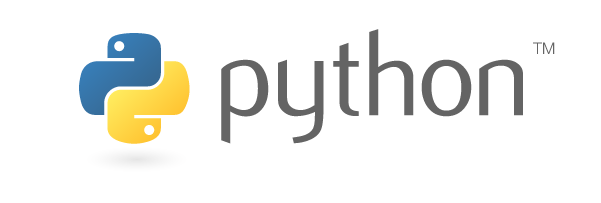
\includegraphics[]{images/python-logo-master-v3-TM-flattened.png}}
\begin{itemize}
    \item Данилов Константин
    \item kdanilov@mirantis.com
\end{itemize}
\newpage
%-------------------------------------------------------------------------------
\center{Почему Python (-)}
\begin{itemize}
    \item Python достаточно сложен для изучения, особенно если разбираться во всех тонкостях
    \item Невозможность качественного статического анализа
    \item Слабая поддержка инструментальными средствами (по сравнению с С++/С\#/Java)
    \item Несколько десятков способов официальных способов выстрелить себе в ногу (и попасть в голову соседу)
    \item Низкая скорость исполнения (по сравнению с компилируемыми языками)
    \item Высокая сложность написания JIT (по сравнению с Javascript)
    \item Поддержку многих высокоуровневых возможностей сложно сделать эффективной 
          == она скорее всего всегда будет медленной
            (перегрузка функций, поиск по образцу, оптимизацию хвостовой рекурсии)
    \item В дизайне языка допускаются ошибки
\end{itemize}
\newpage

%-------------------------------------------------------------------------------
\center{Почему Python (+)}
\begin{itemize}
    \item ~Второй по лаконичности язык (уступает Perl) при этом имея строгий 
            минималистичный синтаксис. Требует значительно меньше кода, чем компилируемые языки.
    \item Ядро языка чрезвычайно компактно. Нет декларируемых конструкций. 
            Все они - синтаксический сахар для исполняемых
    \item В несколько десятков строк можно реализовать большинство отсутствующих языковых возможностей 
    \item Все это + интроспекция = pythonic библиотеки 
        (документация по библиотеке умещается на заглавной странице сайта)
    \item Батарейки в комплекте
    \item Переносимость, обратная совместимость, прогнозируемая и формализованная модель разработки, ...
\end{itemize}
\newpage

%-------------------------------------------------------------------------------
\center{import antigravity}
\begin{itemize}
    \item \lstinline!import antigravity! (python 2.7+)
\end{itemize}
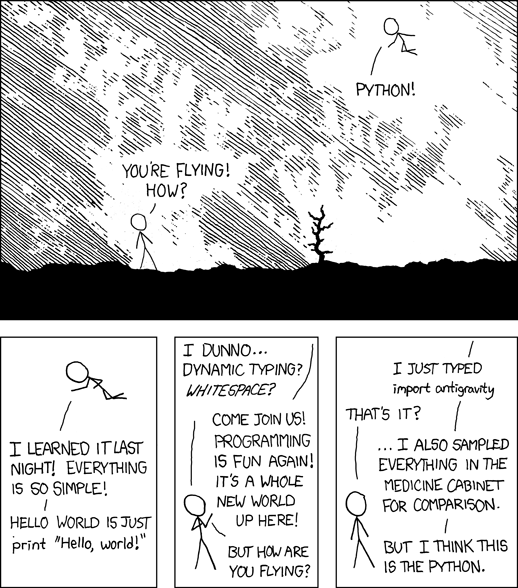
\includegraphics[scale=0.6]{files/antigravity.png}
\newpage

%-------------------------------------------------------------------------------
\center{Python}
\begin{itemize}
    \item Язык программирования ориентированный на скорость работы программиста и
        быстрое освоение библиотек/легкое использование
    \item Мультипарадигменный - процедурный, ООП, функциональный. Позволяет легко реализовывать другие парадигмы
    \item Opensource - hg clone http://hg.python.org/cpython
    \item Monty Python's flying circus
    \item С-подобный минималистичный (учитывая уровень языка) строгий синтаксис
    \item Разрабатывается с конца 80х. В 2001 выходит v2.1 и создается PSF.
    \item Развивается открытым сообществом под руководством Гвидо Ван Россума
    \item Роль стандарта выполняет CPython http://www.python.org
\end{itemize}
\newpage

%-------------------------------------------------------------------------------
\center{Распространение}
\begin{itemize}
    \item ~4-8й язык по популярности (Javascript/VisualBasic/ObjectiveC/PHP)
    \item Научные расчеты и постобработка данных
    \item Web
    \item GUI, Системы управления, встраиваемый язык
    \item Склеивание компонентов, написанных на С/С++
    \item Xen, apt, mercurial, Trac, youtube, GAE, .....
\end{itemize}
\newpage

%-------------------------------------------------------------------------------
\center{Версии и реализации}
\begin{itemize}
    \item Две ветви 2.X(2.7.3) и 3.X(3.3.0rc1) 3.3.0 запланирована на 22 сентября
    \item 2.8 не будет
    \item Внутри каждой ветви поддерживается полная обратная совместимость (для py файлов)
    \item 3.X (Python 3k) достаточно близка к 2.Х, содержит несовместимые исправления 
    		архитектурных ошибок, внесенных в язык на ранних стадиях
    \item print стал функцией, переработка юникод подсистемы, ввода-вывода и др
    \item Тем не менее любая нетривиальная программа на 2.X должна быть изменена для запуска на 3.X
    \item Все реализации в значительноы мере - интерпретаторы
    \item jython, PyPy, IronPython, Stackless Python, ....
    \item Работает на всех распространенных платфрмах - Intel win/lin/mac/bsd/.., Sun, Power, 
    		ARM(Android), Symbian, .....
\end{itemize}
\newpage

%-------------------------------------------------------------------------------
\center{Процесс разработки языка}
\begin{itemize}
    \item Формализованный и бюрократический подход к изменениям в языке
    \item Новые версии каждые 1.5 года
    \item Разработка ведется через python-dev \& python-ideas списки рассылки
    \item Все рассылки открытые
    \item Все изменения и предложения описаны в PEP's (Python Enhancement Proposals) 
            в т.ч. и отклоненные
    \item python-ideas -> python-dev -> PEP XXXX -> ... -> {accepted/rejected} by Guido
\end{itemize}
\newpage

%-------------------------------------------------------------------------------
\center{Библиотеки}
\begin{itemize}
    \item Очень широкий спектр библиотек
    \item Web, Сети, DB, Визуализация, Научные расчеты, XML, GUI,...
    \item Есть привязки почти для всех крупных C/C++ библиотек
    \item Cython, SWIG, SIP,...
\end{itemize}
\newpage

%-------------------------------------------------------------------------------
\center{Установка windows}
\begin{itemize}
    \item Windows: 2.7.3 с http://www.python.org/download/ 
    или ActivePython c http://www.activestate.com/activepython/downloads
    \item Почти все библиотеки - http://pypi.python.org/pypi
    \item Ручная установка библиотеки - exe или распаковать zip, и python setup.py install
    \item Пакетные менеджеры - pip, setuptools \\
    	pip или easy\_install install имя\_пакета==версия
    \item virtualenv - создание изолированных окружений
    \item C:{\textbackslash}Python2.7{\textbackslash}lib{\textbackslash}site-packages
\end{itemize}
\newpage

%-------------------------------------------------------------------------------
\center{Установка linux}
\begin{itemize}
    \item Linux: apt-get install python python-setuptools python-pip python-virtualenv
    \item Почти все библиотеки - http://pypi.python.org/pypi
    \item Ручная установка библиотеки - exe или распаковать zip, и python setup.py install
    \item Пакетные мененджеры - pip, setuptools \\
        pip или easy\_install install имя\_пакета==версия
    \item virtualenv - создание изолированных окружений
    \item /usr/lib/python2.7/dist-packages
\end{itemize}
\newpage

%-------------------------------------------------------------------------------
\center{IDE \& Co}
\begin{itemize}
    \item Eclipse + pydev, PyCharm, PyScripter, Python for VS, ...
    \item Notepad++, Sublime Text 2, Texmate
    \item ipython (pyreadline, http://ipython.org/pyreadline.html)
    \item ipython notebook (pyzmq + tornado)
    \item ipython qtconsole (PyQt4)
    \item PEP8, pylint >= pychecker >= pyflakes
    \item winpdb (требует wxpython)
    %\item Все это можно скачать с ......
\end{itemize}
\newpage

%-------------------------------------------------------------------------------
\center{Интерпретатор}
\begin{itemize}
    \item python
    \item ipython
    \item ipython notebook
\end{itemize}
\newpage

%-------------------------------------------------------------------------------
\center{Программа на Python}
\begin{itemize}
    \item Набор файлов на Python
    \item Каждый файл рассматривается как набор строк
\end{itemize}
\center{Заголовок программы}
\vspace{15pt}
\begin{lstlisting}
    #!/usr/bin/env python
    # -*- coding:utf8 -*-
\end{lstlisting}

\begin{itemize}
    \item Часть строки после \# - комментарий
    \item Длинные строки можно переносить, поставив в конце 
    		"\textbackslash". После него не должно идти пробелов
\end{itemize}
\newpage

%-------------------------------------------------------------------------------
\center{Пример программы}
\vspace{15pt}
\begin{lstlisting}
    #!/usr/bin/env python
    # -*- coding:utf8 -*-
    x = 1
    print "Hello, world!"
    print "x =", x
    print "This is definitelly " + \
            "too long line"
\end{lstlisting}
\newpage

%-------------------------------------------------------------------------------
\center{Исполнение программы}
\begin{itemize}
    \item При первой загрузке программа компилируется в байтокод для 
    	виртуального стекового процессора, встроенного в CPython
    \item .py -> .pyc (python compiled)
    \item python -o  .py -> .pyo. Удаление assert, etc
    \item .pyd, .so - бинарные модули
\end{itemize}
\newpage

%-------------------------------------------------------------------------------
\center{Print}
\begin{itemize}
    \item Вывод набора значений или переменных на экран
    \item Автоматически вставляет пробелы между значениями и перенос строки в конце
\end{itemize}
\vspace{15pt}
\begin{lstlisting}
    print var1, var2
    print 1, 2, "34"
    print x, y, x + y
    print x, y, x + y, # no new line
\end{lstlisting}
\newpage

%-------------------------------------------------------------------------------
\center{Внешние модули}
\begin{itemize}
    \item Библиотеки на Python называются модулями или пакетами
    \item \lstinline$import module$ подключает модуль "module" в программу. 
    После этого его элементы доступны как "module.name"
    \item \lstinline$from module import *$ напрямую включает все элементы "module" в программу. 
    \item \lstinline$from module import xxx,yyy$
        напрямую включает выбранные элементы "module" в программу. 
\vspace{15pt}

\begin{lstlisting}
    import os
    from os import listdir
    from os import *

    print os.listdir(".")
\end{lstlisting}
\end{itemize}
\newpage

%-------------------------------------------------------------------------------
\center{Ошибки}
\begin{itemize}
    \item При возникновении ошибки python порождает исключение, 
    			передающееся вверх по стеку до первого обработчика.
    \item Если в программе не определен ни один обработчик ошибок этого типа, то исключение
    			передается в обработчик по умолчанию, печатающий информацию о исключении
    			и завершающий программу.
\end{itemize}

{
\Large
\begin{lstlisting}
    def f1(a, b):
        return a / b

    def f2(m):
        return f1(2, m)

    f2(0)
\end{lstlisting}

\begin{verbatim}
    Traceback (most recent call last):
      File "/tmp/m.py", line 7, in <module>
        f2(0)
      File "/tmp/m.py", line 5, in f2
        return f1(2, m)
      File "/tmp/m.py", line 2, in f1
        return a / b
    ZeroDivisionError: integer division or modulo by zero
\end{verbatim}
}

\newpage

%-------------------------------------------------------------------------------
\center{Справка и исследование объектов}
\begin{itemize}
    \item help(obj)
    \item obj?    -- help
    \item obj??   -- help + source
    \item obj.<tab>  -- extension
    \item dir(obj)
\end{itemize}

\begin{lstlisting}
    In [1]: import antigravity

    In [2]: antigravity??
    Type:       module
    String Form:<module 'antigravity' from 'C:\Dev\Python\Python27_x86\lib\antigravity.py'>
    File:       c:\dev\python\python27_x86\lib\antigravity.py
    Source:

    import webbrowser

    webbrowser.open("http://xkcd.com/353/")
\end{lstlisting}
\newpage

%-------------------------------------------------------------------------------
\center{Документация по python}
\begin{itemize}
    \item Идет с питоном
    \item python.org
    \item Г. Россум, Ф.Л.Дж. Дрейк, Д.С. Откидач Язык программирования Python
    \item http://slav0nic.org.ua/static/books/python/
    \item http://rutracker.org/forum/viewtopic.php?t=2436308
    \item http://www.python.ru/docs/
\end{itemize}
\newpage

%-------------------------------------------------------------------------------
\center{AA}
\begin{itemize}
    \item Установить Python
    \item Создать виртуальное окружение для python, 
            вся дальнейшая работа будет идти из него
    \item Установить ipython (со всеми зависимостями)
    \item ipython qtconsole, ipython notebook
    \item аккаунт на pikacode + mercurial + TortoiseHG
    \item или аккаунт на github + git (привет, windows!)
    \item sublime text 2 / notepad++ / vim / emacs /eclipse + pydev
    \item Найти и прочитать pep8
    \item \lstinline!import this! - the Zen of Python
    \item pep8 + pylint
    \item winpdb
\end{itemize}
\newpage

%-------------------------------------------------------------------------------
\end{document}
